\documentclass[aspectratio=43, 10pt]{beamer}
\usepackage[utf8]{inputenc}
\usepackage[T1]{fontenc}
\usepackage{helvet}
\usepackage{graphicx}
\usepackage{tikz}
\usepackage{booktabs}
\usepackage{xcolor}

% Theme
\usetheme{metropolis}
\usecolortheme{default}
\setbeamercolor{structure}{fg=darkgray} 
\setbeamercolor{frametitle}{bg=white, fg=black}
\setbeamertemplate{navigation symbols}{}
\setbeamertemplate{footline}[frame number]

% Infos
\graphicspath{{images/}}
\title{Modeling Insurance Risk with Self-Exciting Processes}
\subtitle{Why Standard Poisson Models Underestimate Ruin Probability}
\author{Driss Chraibi \and Wassim Fathi \and Paul Louka}
\institute{INSA Toulouse, ENSEEIHT - ModIA 2\textsuperscript{nd} Year}
\date{November 2025}

\begin{document}

\begin{frame}
    \titlepage
    \vspace*{-5em}
    \begin{center}
        \small Prepared for the Risk Management Board
    \end{center}
\end{frame}

% PART 1: CONTEXT (Speaker: Driss)
% Goal: Hook the insurance company. Standard models fail for contagion events.
\begin{frame}{Standard models underestimate the risk of contagion}
    
    \begin{columns}
        \column{0.5\textwidth}
        \textbf{The Status Quo (Poisson)}
        \begin{itemize}
            \item Assumes claims are \textbf{independent}.
            \item Good for: Car accidents, house fires.
            \item \alert{Fails for:} Epidemics, natural disasters, chain collisions.
        \end{itemize}
        
        \vspace{1em}
        \textbf{The Reality}
        \begin{itemize}
            \item Events cluster in time.
            \item One claim increases the probability of the next.
        \end{itemize}
        
        \column{0.5\textwidth}
        \centering
        % Visual representation of clustering vs independence
        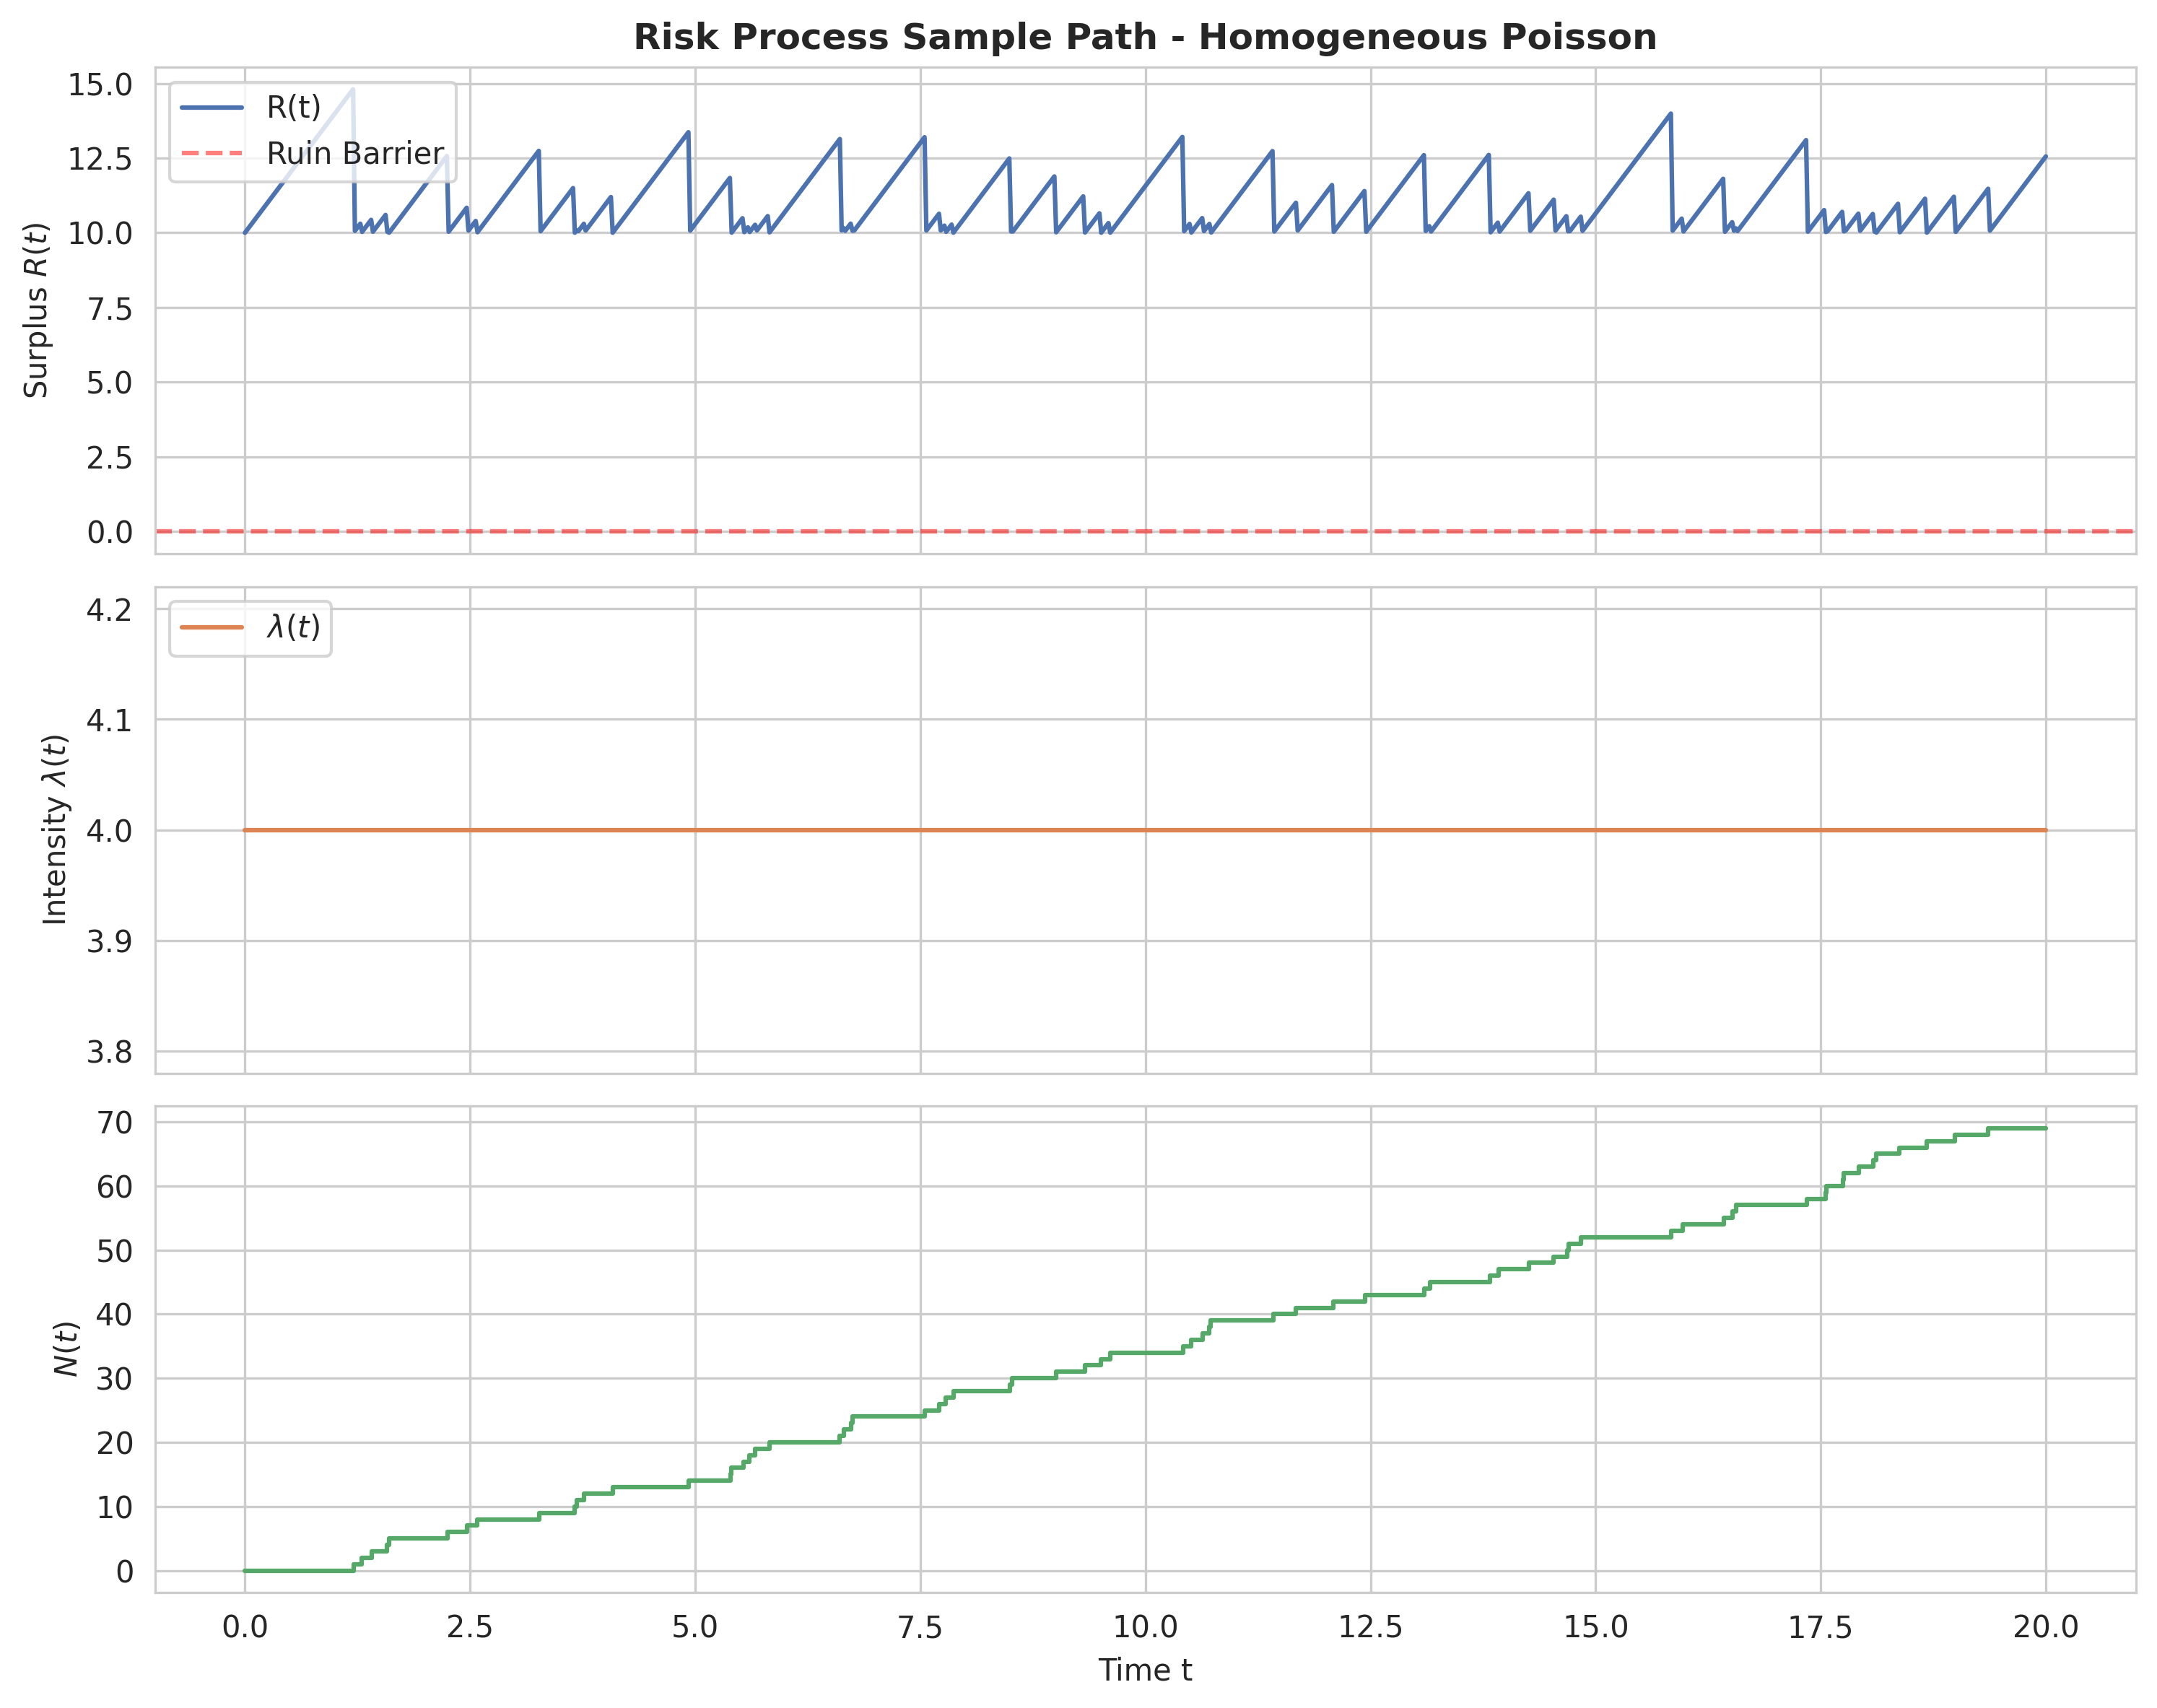
\includegraphics[width=0.6\textwidth]{path_hpp.png} \\
        \textit{vs.} \\
        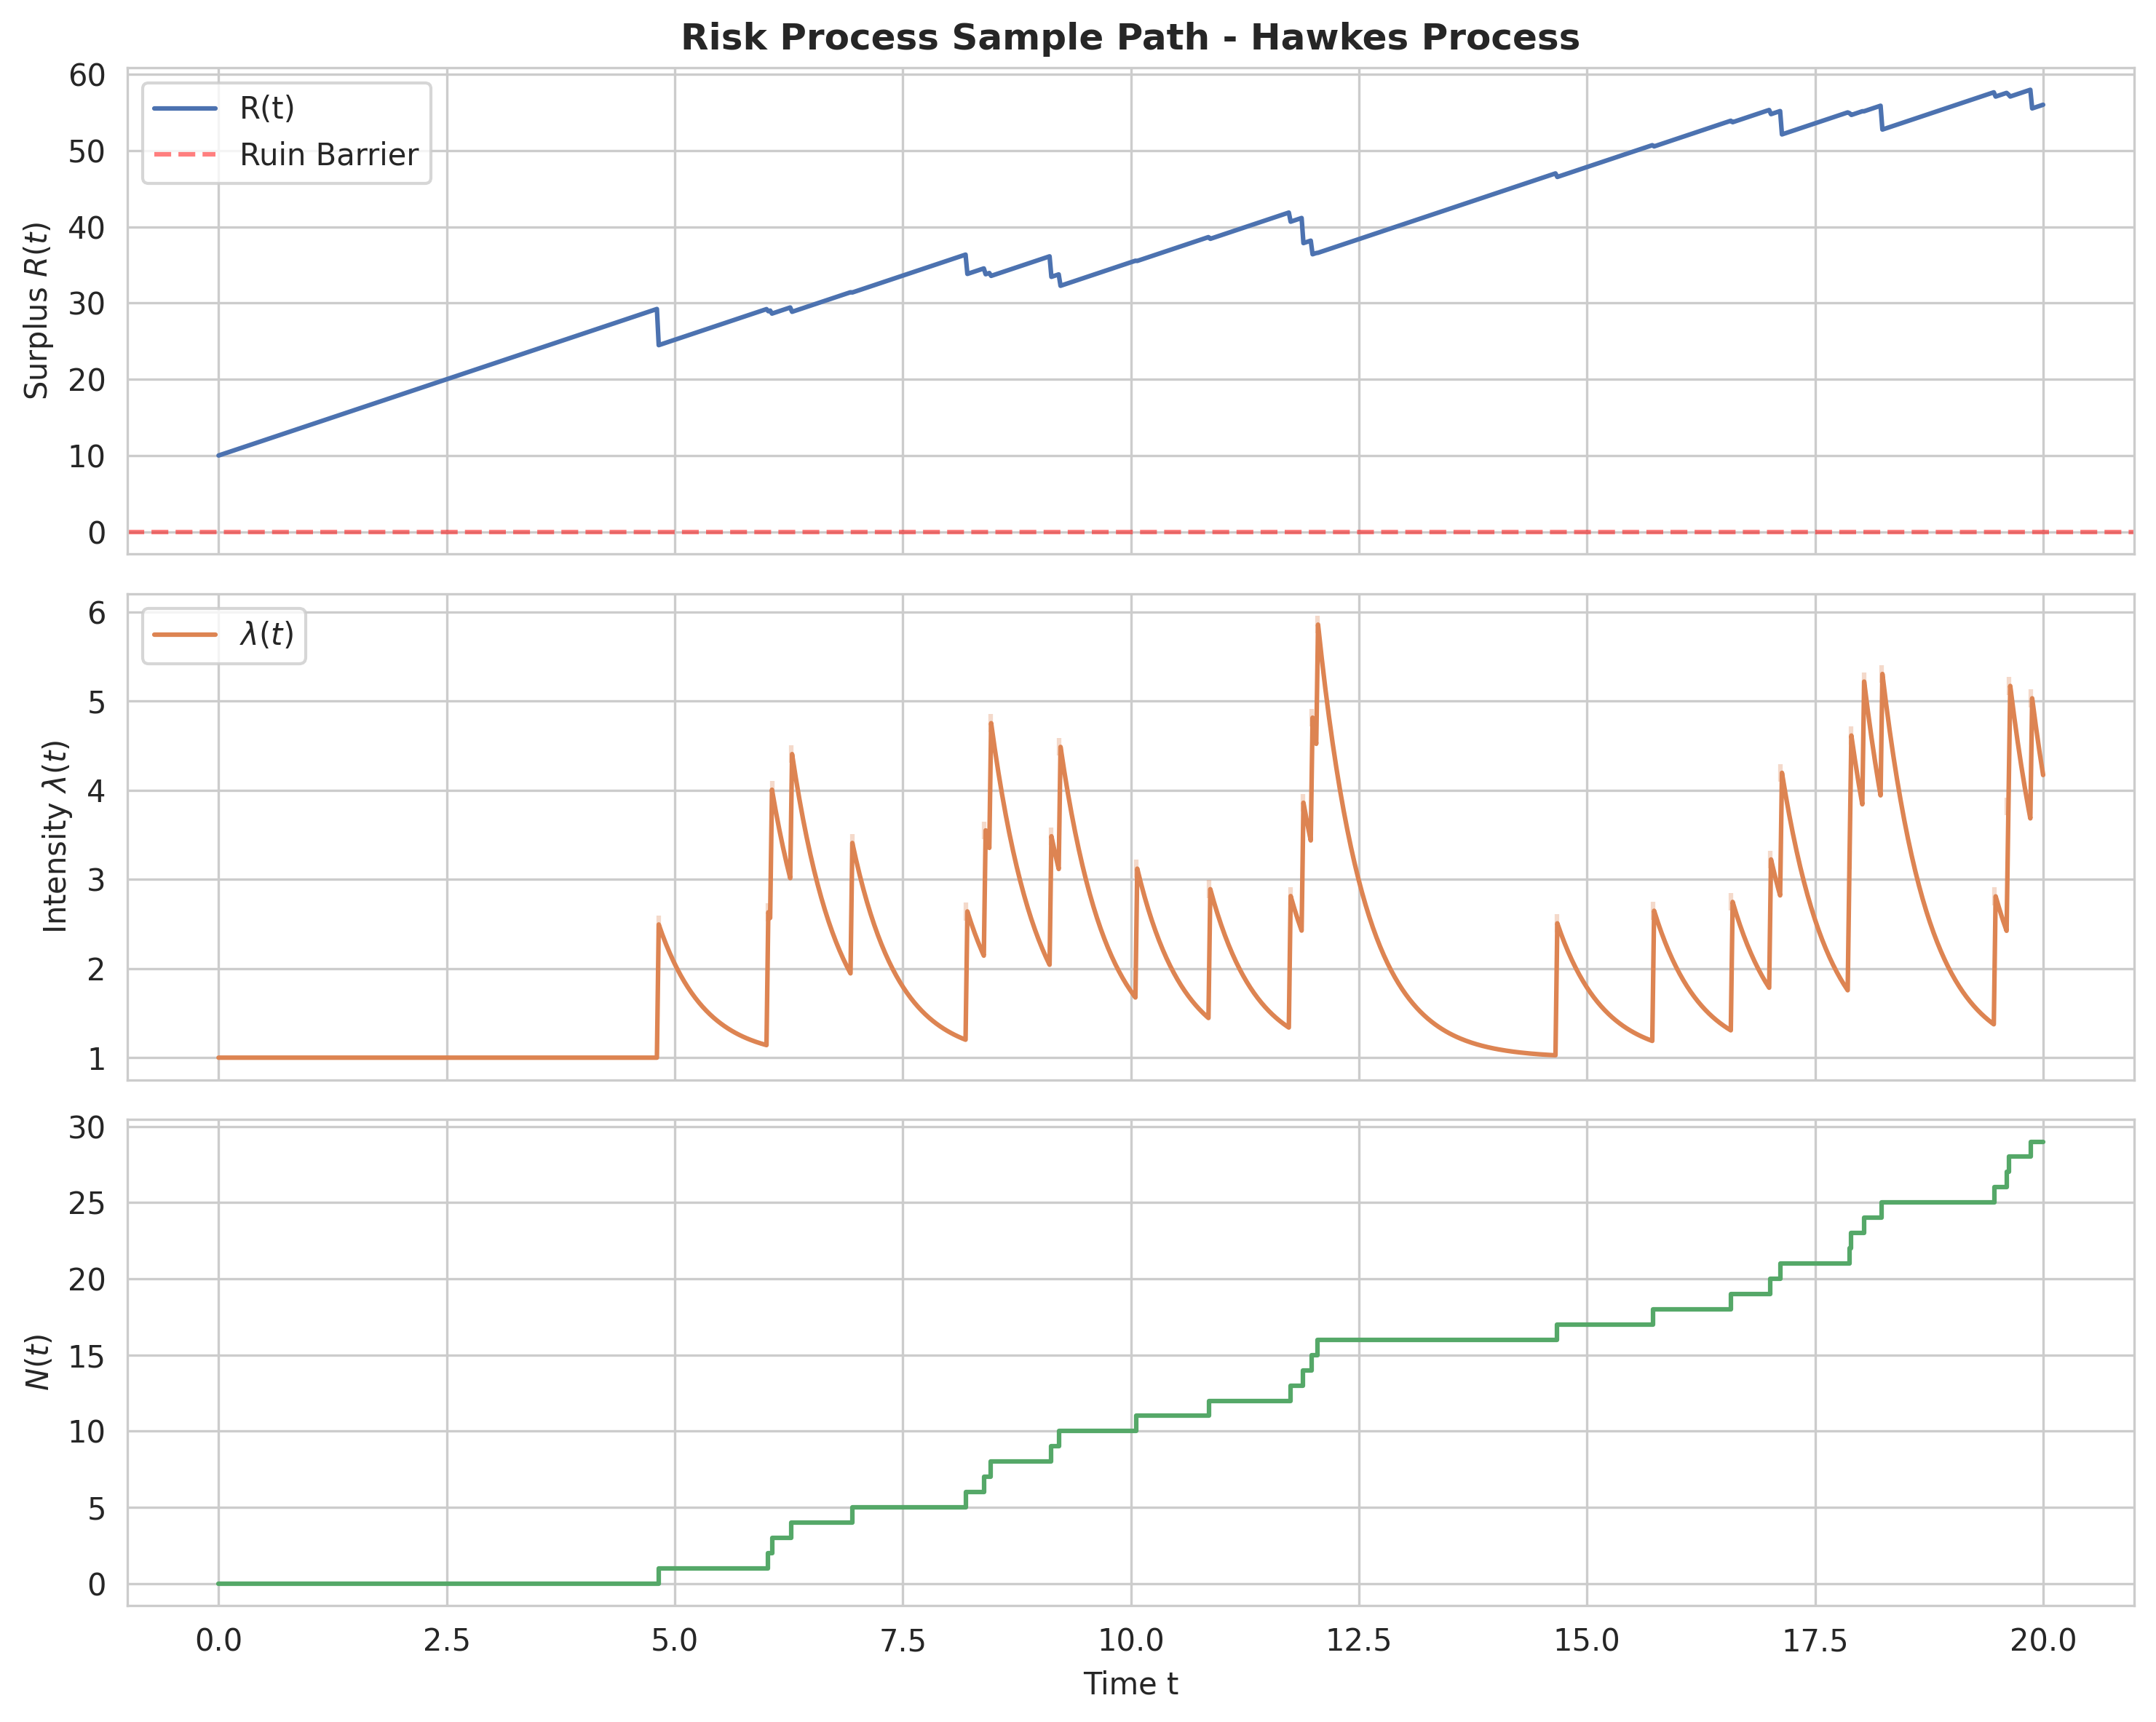
\includegraphics[width=0.6\textwidth]{path_hawkes.png}
    \end{columns}
\end{frame}

\begin{frame}{The Cramér-Lundberg model must adapt to history}

    The classical surplus equation:
    $$ R(t) = u + ct - \sum_{i=1}^{N(t)} X_i $$
    
    \vspace{1em}
    
    \begin{columns}
        \column{0.6\textwidth}
        \begin{itemize}
            \item \textbf{$u$}: Initial Capital (Reserves).
            \item \textbf{$c$}: Premium Rate (Income).
            \item \textbf{$N(t)$}: \alert{The weak link.}
        \end{itemize}
        \vspace{1em}
        If $N(t)$ ignores history, we misprice the risk of ruin.
        
        \column{0.4\textwidth}
    \end{columns}
\end{frame}

% PART 2: THE MODEL (Speaker: Wassim)
% Goal: Explain Hawkes simply. Focus on "Self-excitation" and the "Mean Trap".
\begin{frame}{Hawkes processes capture the "Aftershock" effect}
    
    The intensity $\lambda(t)$ is not constant; it reacts to history.
    
    $$ \lambda(t) = \mu + \sum_{t_i < t} \alpha e^{-\beta(t - t_i)} $$
    
    \vspace{1em}
    
    \begin{columns}
        \column{0.5\textwidth}
        \textbf{Key Mechanics:}
        \begin{itemize}
            \item \textbf{$\mu$}: Baseline risk (day-to-day).
            \item \textbf{Jump ($\alpha$)}: Sudden panic/contagion.
            \item \textbf{Decay ($\beta$)}: System recovery speed.
        \end{itemize}

        \column{0.5\textwidth}
        \centering
        % Use the intensity plot from the report
        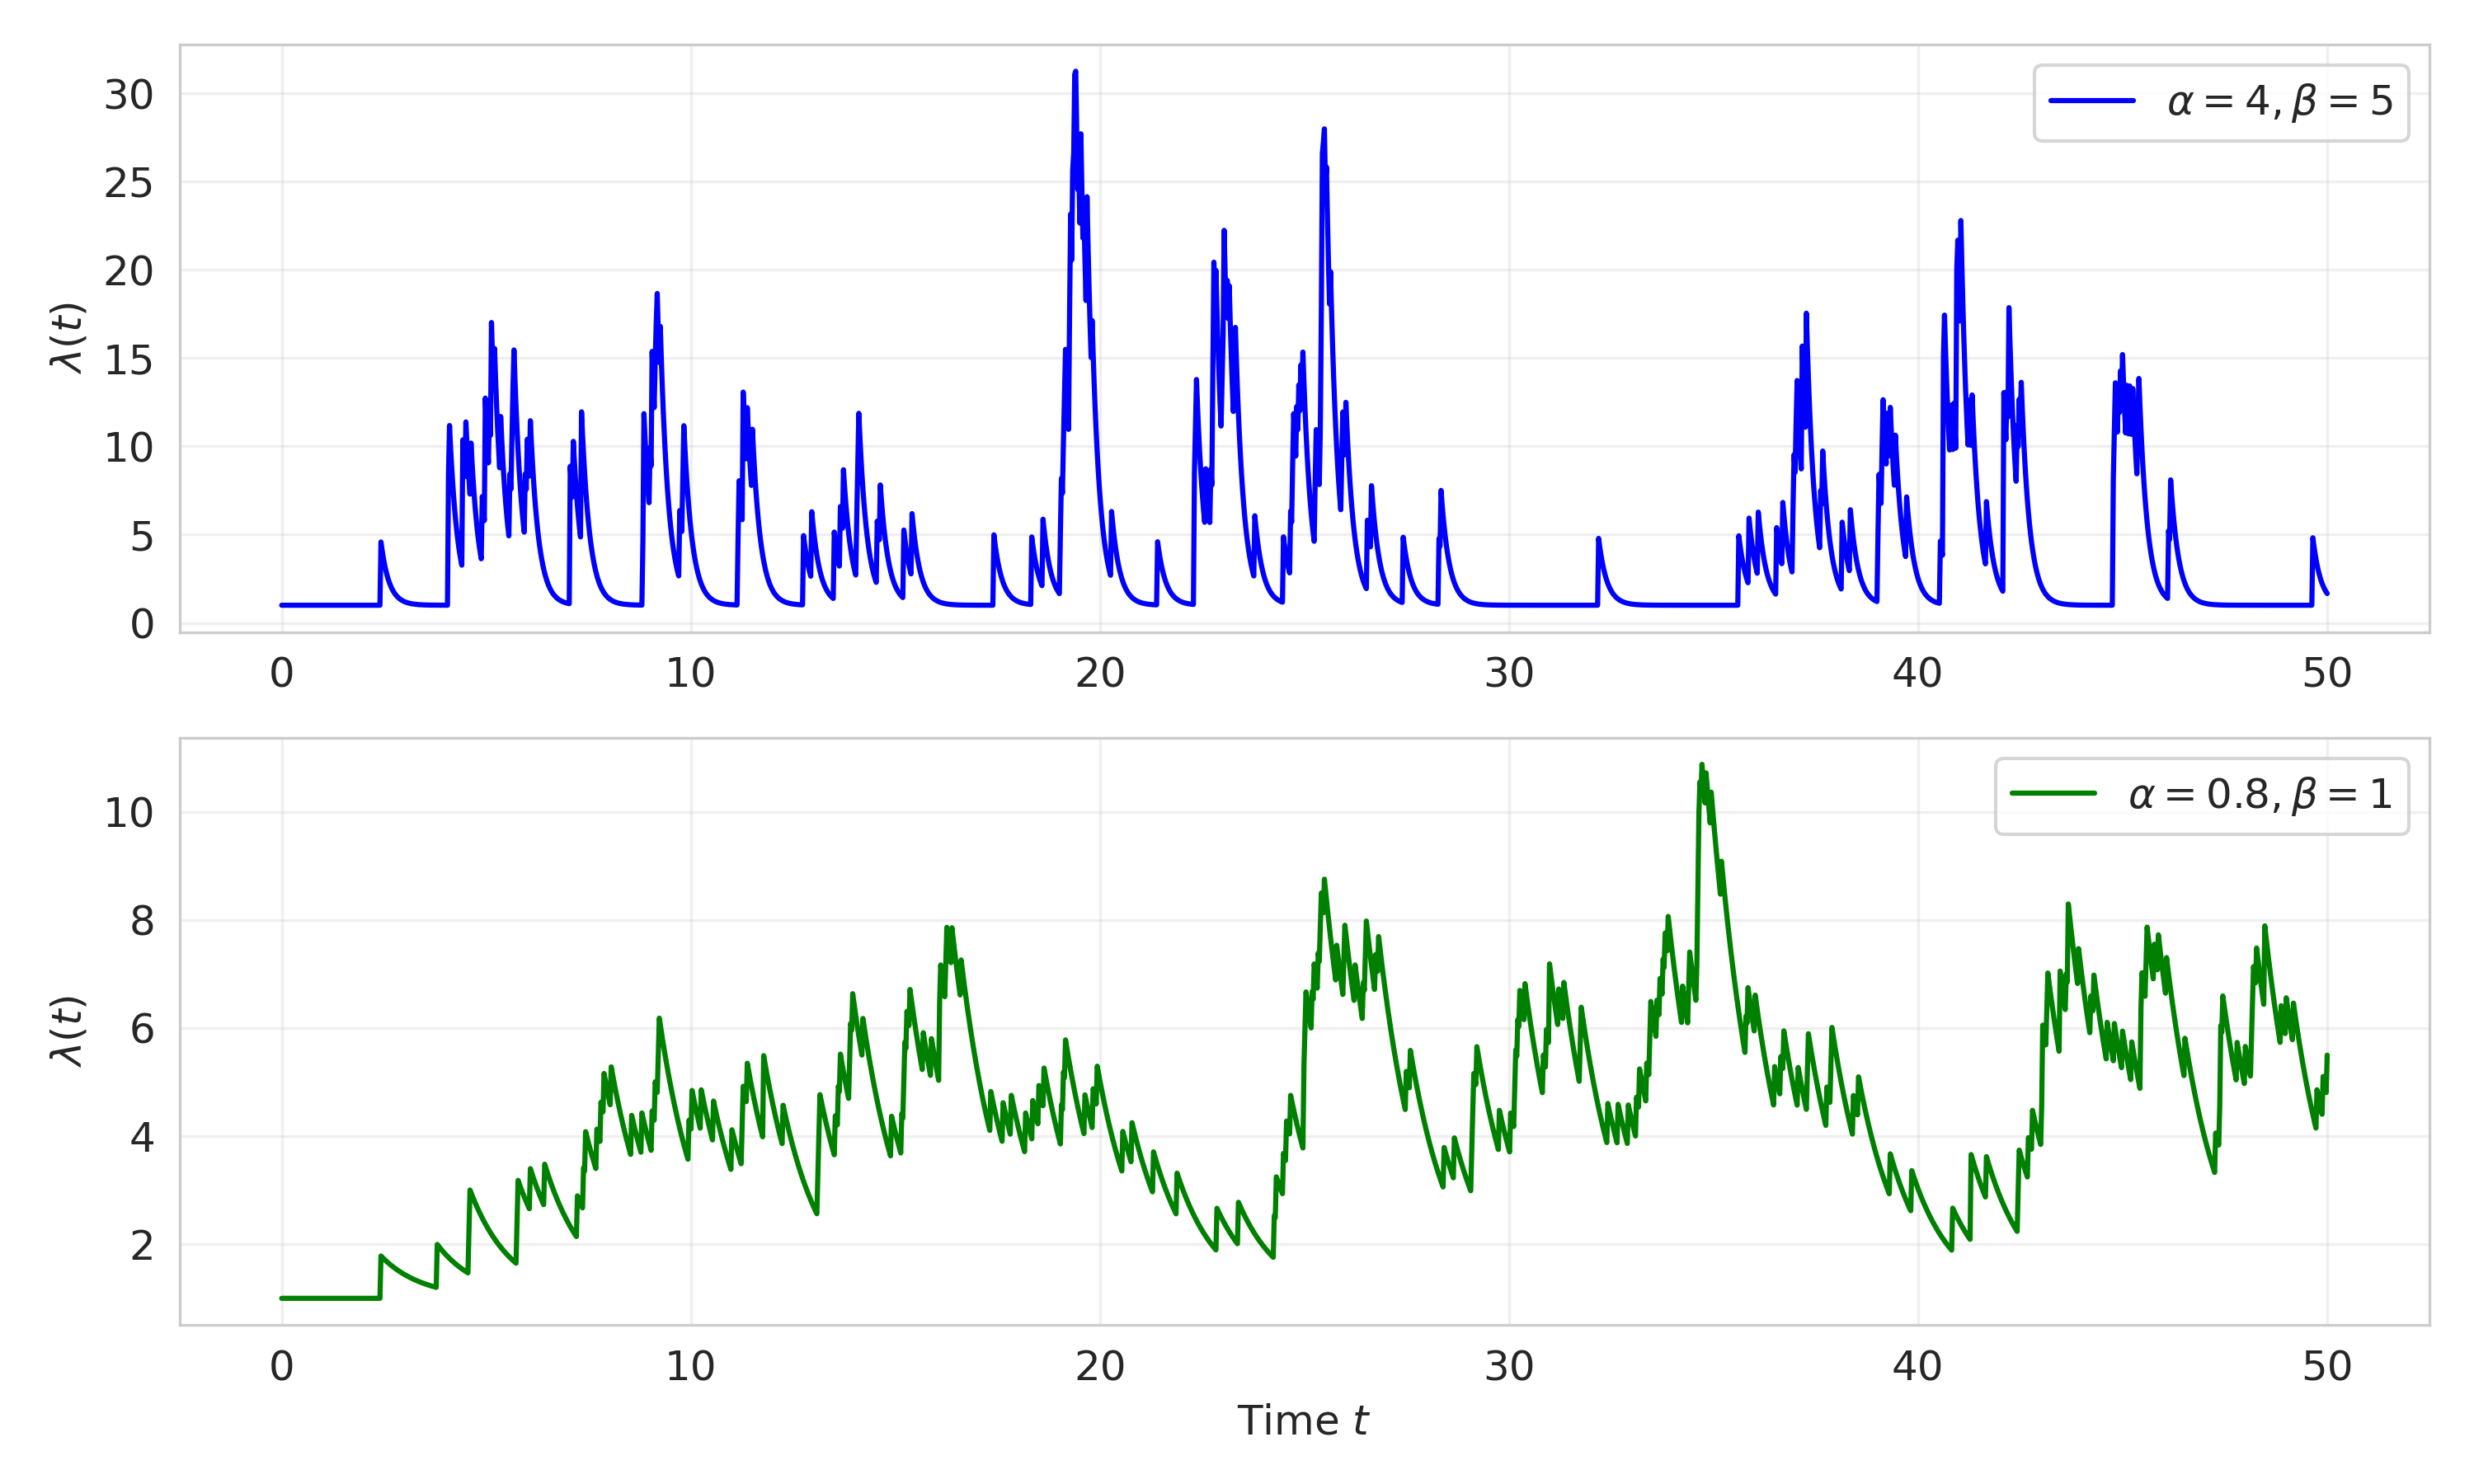
\includegraphics[width=\textwidth]{intensity_influence.png}
    \end{columns}
\end{frame}

\begin{frame}{Average profitability does not guarantee solvency}
    
    \begin{block}{The Net Profit Condition (NPC)}
        $$ c > \frac{\mu}{1-n} \cdot \mathbb{E}[X] $$
    \end{block}
    
    \vspace{0.5cm}
    
    \begin{itemize}
        \item \textbf{The Trap:} Two models can have the \textbf{same average} number of claims but vastly different risks.
        \item \textbf{The Danger:} Stability depends on the branching ratio $n = \alpha/\beta < 1$.
        \item Meeting the NPC is \textbf{necessary, but not sufficient}.
    \end{itemize}
\end{frame}

% PART 3: SIMULATION & RISK (Speaker: Paul)
% Goal: Show the "Fat Tails" and clustering visuals.
\begin{frame}{We use Ogata's Algorithm to simulate path-dependence}

    Since risk changes every second, standard simulations fail.
    
    \vspace{1em}
    
    \begin{columns}
        \column{0.5\textwidth}
        \textbf{Methodology:}
        \begin{enumerate}
            \item Simulate a "worst-case" rate $\lambda^*$.
            \item Rejection sampling based on history.
            \item Exact simulation (no bias).
        \end{enumerate}

        \column{0.5\textwidth}
        \centering
        % Visual aid for the algorithm (conceptual)
        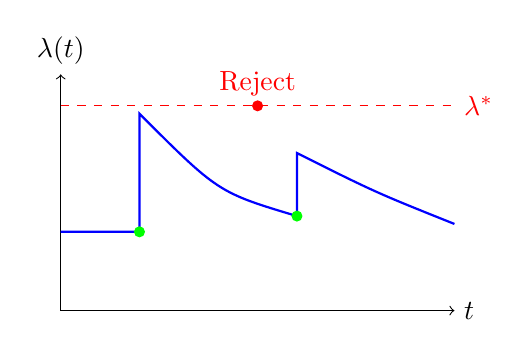
\begin{tikzpicture}
            \draw[->] (0,0) -- (5,0) node[right] {$t$};
            \draw[->] (0,0) -- (0,3) node[above] {$\lambda(t)$};
            \draw[thick, blue] (0,1) -- (1,1) -- (1,2.5) .. controls (2,1.5) .. (3,1.2) -- (3,2.0) .. controls (4,1.5) .. (5,1.1);
            \draw[dashed, red] (0,2.6) -- (5,2.6) node[right] {$\lambda^*$};
            \fill[red] (2.5, 2.6) circle (2pt) node[above] {Reject};
            \fill[green] (1, 1) circle (2pt);
            \fill[green] (3, 1.2) circle (2pt);
        \end{tikzpicture}
    \end{columns}
\end{frame}

\begin{frame}{Clustering creates dangerous "Fat Tails"}
    
    Comparing Poisson vs. Hawkes with the \textbf{same mean} ($\mathbb{E}[N]=250$).
    
    \begin{center}
        
\includegraphics[width=0.75\textwidth]{clustering_histogram.png}
    \end{center}
    
    \begin{itemize}
        \item \textcolor{blue}{Poisson}: Predictable, bell-shaped.
        \item \textcolor{red}{Hawkes}: High probability of \textbf{extreme scenarios}.
    \end{itemize}
\end{frame}

% IMPACT & SOLUTION (Speaker: Driss)
% Goal: The financial results. Hawkes = Higher Ruin. Solution = Reinsurance.
\begin{frame}{Hawkes models reveal hidden bankruptcy risks}

    Probability of Ruin $\psi(u)$ vs. Premium $c$.
    
    \begin{columns}
        \column{0.5\textwidth}
        \begin{itemize}
            \item \textbf{Solvent Zone ($c > c_{min}$)}:
            \item Poisson model predicts safety (Blue).
            \item Hawkes model predicts \textbf{ruin} (Red).
            \item \alert{Result:} Reserves calculated on Poisson are insufficient.
        \end{itemize}

        \column{0.5\textwidth}
        \centering
        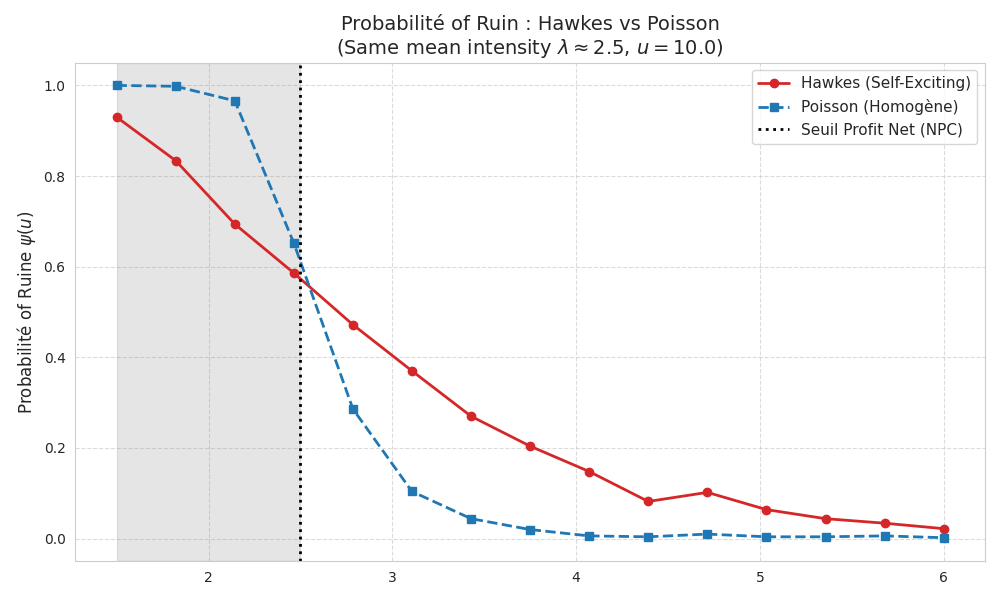
\includegraphics[width=\textwidth]{ruin_hawkes_vs_poisson.png}
    \end{columns}
\end{frame}

\begin{frame}{Stop-Loss Reinsurance mitigates the clustering risk}

    We transfer the "Tail Risk" to a reinsurer.
    
    $$ I_t = \min(S_t, P) $$
    
    \begin{columns}
        \column{0.6\textwidth}
        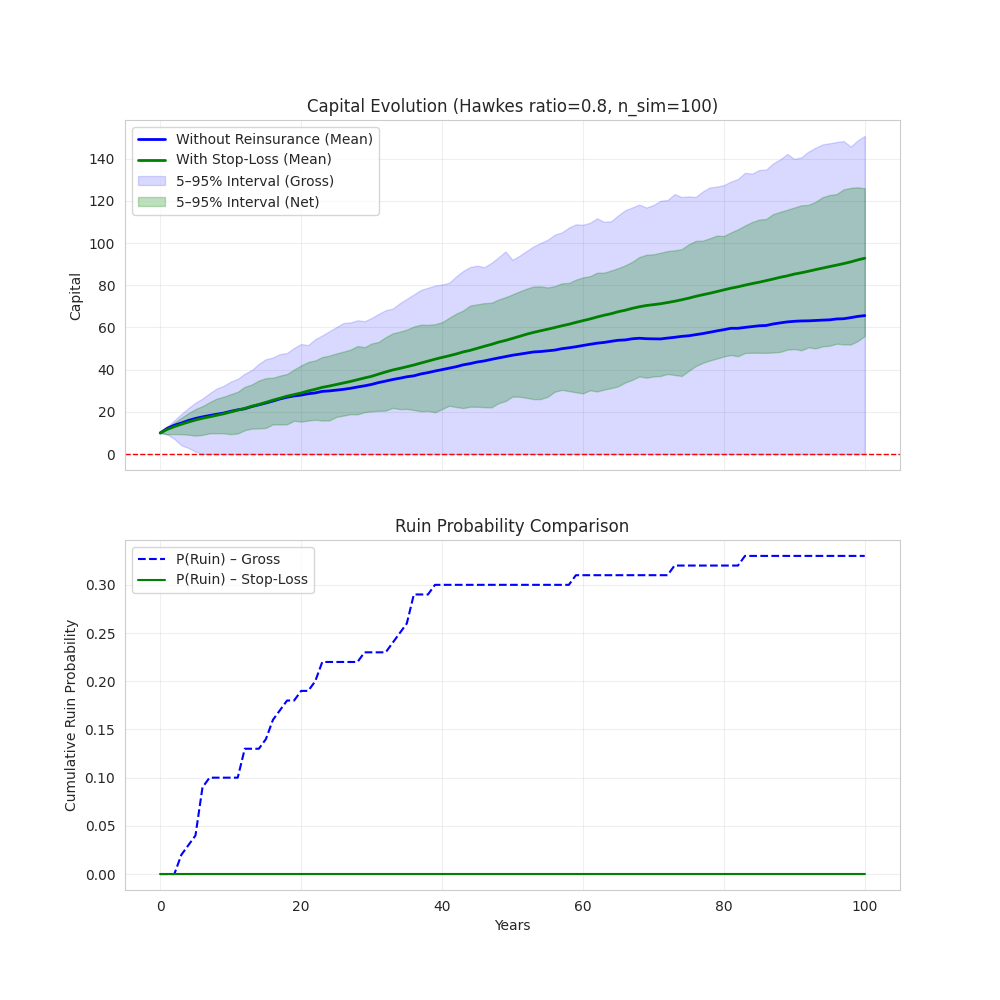
\includegraphics[width=\textwidth]{reinsurance.png}
        
        \column{0.4\textwidth}
        \textbf{Outcome:}
        \begin{itemize}
            \item \textcolor{blue}{Blue (Gross)}: High volatility, ruin probable.
            \item \textcolor{green}{Green (Net)}: Stable growth, ruin eliminated.
        \end{itemize}
    \end{columns}
\end{frame}

\begin{frame}{Recommendation}
    \textbf{Conclusion}
    
    \begin{enumerate}
        \item \textbf{Acknowledge Contagion:} Standard models dangerously underestimate variance.
        \item \textbf{Monitor Parameters:} $\alpha$ (Jump) and $\beta$ (Memory) are as important as the mean.
        \item \textbf{Purchase Protection:} Capital reserves alone are inefficient; Stop-Loss reinsurance is required for stability.
    \end{enumerate}
    
    \vspace{1cm}
    \centering
    \large \textbf{Do you have any questions?}
\end{frame}

\begin{frame}[allowframebreaks]{References}
    \tiny
    \bibliographystyle{plain}
    \begin{thebibliography}{9}
        \bibitem{hawkes1974} Hawkes, A. G., \& Oakes, D. (1974). A cluster process representation of a self-exciting process. \textit{Journal of Applied Probability}.
        \bibitem{bacry2015} Bacry, E., et al. (2015). Hawkes processes in finance. \textit{Market Microstructure and Liquidity}.
        \bibitem{ogata1981} Ogata, Y. (1981). On Lewis' simulation method for point processes. \textit{IEEE Transactions}.
    \end{thebibliography}
\end{frame}

\end{document}
